\providecommand{\Person}[1]{
\draw[ultra thick] (#1) circle (.4cm);
}
\providecommand{\Exposed}[1]{
\draw[ultra thick,fill=gray!50] (#1) circle (.4cm);
}
\providecommand{\Sick}[1]{
\draw[ultra thick] (#1) -- +(.25,.25);
\draw[ultra thick] (#1) -- +(.25,-.25);
\draw[ultra thick] (#1) -- +(-.25,-.25);
\draw[ultra thick] (#1) -- +(-.25,.25);
}
\providecommand{\PersonSick}[1]{
\Person{#1}
\Sick{#1}
}
\providecommand{\ExposedSick}[1]{
\Exposed{#1}
\Sick{#1}
}

The diagrams below show different diseases along with exposure to
some hypothesized cause.  

{\bf Key}: Each circle is a person who might or might not have been exposed to the hypothetical cause and who might or might not have eventually acquired the disease.
\begin{itemize}
\item Exposed but not sick 
\begin{tikzpicture} \Exposed{0,0} \end{tikzpicture}
\item Sick 
\begin{tikzpicture} \PersonSick{0,0} \end{tikzpicture}
\item Exposed and Sick 
\begin{tikzpicture} \ExposedSick{0,0} \end{tikzpicture}
\item Neither exposed nor sick 
\begin{tikzpicture} \Person{0,0} \end{tikzpicture}
\end{itemize}


For each of the diseases, say whether the
exposure is a necessary and/or sufficient cause for development of the disease.

\begin{itemize}
\item Disease C

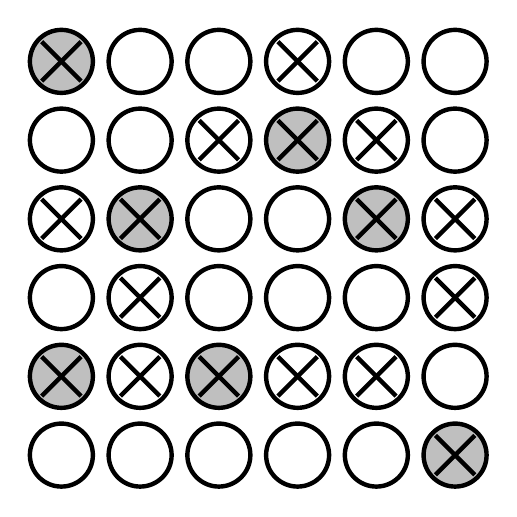
\begin{tikzpicture}
\Person{0,0}\ExposedSick{0,1}\Person{0,2}\PersonSick{0,3}\Person{0,4}\ExposedSick{0,5}
\Person{1,0}\PersonSick{1,1}\PersonSick{1,2}\ExposedSick{1,3}\Person{1,4}\Person{1,5}
\Person{2,0}\ExposedSick{2,1}\Person{2,2}\Person{2,3}\PersonSick{2,4}\Person{2,5}
\Person{3,0}\PersonSick{3,1}\Person{3,2}\Person{3,3}\ExposedSick{3,4}\PersonSick{3,5}
\Person{4,0}\PersonSick{4,1}\Person{4,2}\ExposedSick{4,3}\PersonSick{4,4}\Person{4,5}
\ExposedSick{5,0}\Person{5,1}\PersonSick{5,2}\PersonSick{5,3}\Person{5,4}\Person{5,5}
\end{tikzpicture}


For Disease C

\begin{MultipleChoice}[itemname=nec-and-suff-c]
\correct{Necessary but not sufficient}
\wrong{Sufficient but not necessary}
\wrong{Necessary and Sufficient}
\wrong{Neither necessary nor sufficient}
\end{MultipleChoice}
\end{itemize}

\begin{itemize}

\item Disease D

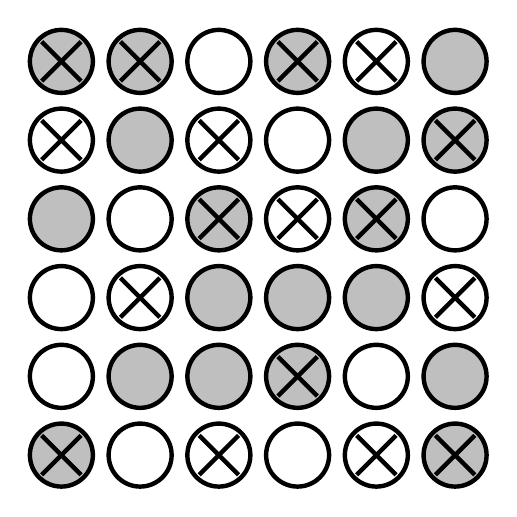
\begin{tikzpicture}
\ExposedSick{0,0}\Person{0,1}\Person{0,2}\Exposed{0,3}\PersonSick{0,4}\ExposedSick{0,5}
\Person{1,0}\Exposed{1,1}\PersonSick{1,2}\Person{1,3}\Exposed{1,4}\ExposedSick{1,5}
\PersonSick{2,0}\Exposed{2,1}\Exposed{2,2}\ExposedSick{2,3}\PersonSick{2,4}\Person{2,5}
\Person{3,0}\ExposedSick{3,1}\Exposed{3,2}\PersonSick{3,3}\Person{3,4}\ExposedSick{3,5}
\PersonSick{4,0}\Person{4,1}\Exposed{4,2}\ExposedSick{4,3}\Exposed{4,4}\PersonSick{4,5}
\ExposedSick{5,0}\Exposed{5,1}\PersonSick{5,2}\Person{5,3}\ExposedSick{5,4}\Exposed{5,5}
\end{tikzpicture}

For Disease D

\begin{MultipleChoice}[itemname=nec-and-suff-d]
\wrong{Necessary but not sufficient}
\wrong{Sufficient but not necessary}
\wrong{Necessary and Sufficient}
\correct{Neither necessary nor sufficient}
\end{MultipleChoice}

\end{itemize}

